\documentclass[final,hyperref={pdfpagelabels=false}]{beamer}
\usepackage{grffile}
\mode<presentation>{\usetheme{I6pd2}}


%\usecolortheme[snowy]{owl} %Yo puse este tema que me gusta.


\usepackage{babel}
\usepackage[latin1]{inputenc}
\usepackage{amsmath,amsthm, amssymb, latexsym}
%\usefonttheme[onlymath]{serif}
\boldmath
\usepackage[orientation=portrait,size=a0,scale=1,debug]{beamerposter}
% change list indention level
% \setdefaultleftmargin{3em}{}{}{}{}{}


%\usepackage{snapshot} % will write a .dep file with all dependencies, allows for easy bundling

\usepackage{array,booktabs,tabularx}
\newcolumntype{Z}{>{\centering\arraybackslash}X} % centered tabularx columns
\newcommand{\pphantom}{\textcolor{ta3aluminium}} % phantom introduces a vertical space in p formatted table columns??!!

\listfiles




%%%%%%%%%%%%%%%%%%%%%%%%%%%%%%%%%%%%%%%%%%%%%%%%%%%%%%%%%%%%%%%%%%%%%%%%%%%%%%%%%%%%%%%%%%%%%%%%%%%%

% custom colors
\definecolor{i6blue}{cmyk}{1,0.305,0,0.06}
\definecolor{i6bluedark}{rgb}{0.0156,0.2578,0.5625} 
\definecolor{i6colorscheme1}{HTML}{261F55}  % e.g. for block title purple
\definecolor{i6colorblockbg}{HTML}{FF69B4}  % hotpink
\definecolor{i6colorblockfg}{HTML}{0A080E}  %purple black
\definecolor{i6colorscheme2}{HTML}{000000}  % e.g. title in headline
\definecolor{i6colorscheme3}{HTML}{DFDFDF}  % e.g. for poster background, gris claro
\definecolor{i6colorscheme4}{HTML}{000000} 
\definecolor{i6colorschemeHeadline}{HTML}{4F4F4F}  % for headline bg
\definecolor{i6colorschemeFootline}{HTML}{100D09}  % for headline bg

% headline colors and fonts
\setbeamercolor{headline}{fg=white,bg=i6colorschemeHeadline}
\setbeamercolor{title in headline}{fg=white}
\setbeamercolor{author in headline}{fg=white}
\setbeamercolor{institute in headline}{fg=lightgray}
\setbeamercolor{logo in headline}{fg=black,bg=lightgray}
\setbeamercolor{separation line}{bg=i6colorscheme1}


% body colors and fonts
\setbeamercolor*{normal text}{fg=black,bg=i6colorscheme3}

% block environment
\setbeamercolor*{block body}{bg=white,fg=black}
\setbeamercolor*{block title}{fg=i6colorblockfg,bg=i6colorblockbg}
\setbeamerfont{block title}{size=\large,series=\bf}

% example environment
\setbeamercolor*{example title}{fg=white,bg=i6colorscheme1}

\setbeamercolor{alerted text}{fg=i6colorscheme1}

\setbeamertemplate{itemize items}[triangle]
\setbeamertemplate{navigation symbols}{}  % no navigation on a poster

%%%%%%%%%%%%%%%%%%%%%%%%%%%%%%%%%%%%%%%%%%%%%%%%%%%%%%%%%%%%%%%%%%%%%%%%%%%%%%%%%%%%%%%%%%%%%%%%%%%%




			%% Símbolos matemáticos
			\newcommand*{\QEDA}{\null\nobreak\hfill\ensuremath{\blacksquare}}%
			\newcommand*{\QEDB}{\null\nobreak\hfill\ensuremath{\square}}%
			\newcommand{\TODO}[1]{\textcolor{purple}{#1}}
			\newcommand*{\final}{\null\nobreak\hfill\ensuremath{\diamond}}
			\newcommand{\IR}{\mathbb{R}}
			\newcommand{\IC}{\mathbb{C}}
			\newcommand{\IN}{\mathbb{N}}
			\newcommand{\IZ}{\mathbb{Z}}
			\newcommand{\suma}[3]{\sum\limits_{#1}^{#2}#3} %Sumas y series
			\newcommand{\union}[3]{\bigcup\limits_{#1}^{#2}{#3}} %uniones
			\newcommand{\producto}[3]{\prod_{#1}^{#2}{#3}} %productos
			\newcommand{\limite}[2]{\lim\limits_{#1}{#2}} %límites
			\newcommand{\limsu}[2]{\lim\limits_{#1 \rightarrow \infty }#2_{#1}}
			%para límites de sucesiones
			\newcommand{\Om}{\Omega}
			\newcommand{\cali}[1]{\mathcal{#1}} %Letras caligráficas
			\newcommand{\cont}[2]{$\mathcal{C} [#1, #2]$}
			\newcommand{\integ}[3]{\int_{#1}^{#2}{#3}}
			\newcommand{\ldos}{\mathit{l}^{2}}



%%%%%%%%%%%%%%%%%%%%%%%%%%%%%%%%%%%%%%%%%%%%%%%%%%%%%%%%%%%%%%%%%%%%%%%%%%%%%%%%%%%%%%
\graphicspath{{figures/}}

\setlogo{logo_BUAP}
\setauthorurl{https://github.com/AmelieBernes/tesis-licenciatura}
\setauthoremail{ammel.bernes@gmail.com}

\title{\huge Estudio y an\'alisis espectral de los polinomios discretos de Legendre}
\author{Am\'elie Bern\`es, Moises Soto y Javier Herrera}
%\institute[BUAP]{Benem\érita Universidad Aut\'onoma de Puebla}
\institute[BUAP]{Benemerita Universidad Autonoma de Puebla}
\date[Sep. 8th, 2009]{Sep. 8th, 2009}


%%%%%%%%%%%%%%%%%%%%%%%%%%%%%%%%%%%%%%%%%%%%%%%%%%%%%%%%%%%%%%%%%%%%%%%%%%%%%%%%%%%%%%
\newlength{\columnheight}
\setlength{\columnheight}{120cm}


%%%%%%%%%%%%%%%%%%%%%%%%%%%%%%%%%%%%%%%%%%%%%%%%%%%%%%%%%%%%%%%%%%%%%%%%%%%%%%%%%%%%%%
\begin{document}
\begin{frame}
  \begin{columns}
    % ---------------------------------------------------------%
    % Set up a column 
    \begin{column}{.49\textwidth}
      \begin{beamercolorbox}[center,wd=\textwidth]{postercolumn}
        %\begin{minipage}[T]{.95\textwidth}  % tweaks the width, makes a new \textwidth
         % \parbox[t][\columnheight]{\textwidth}{ % must be some better way to set the the height, width and textwidth simultaneously
            % Since all columns are the same length, it is all nice and tidy.  You have to get the height empirically
            % ---------------------------------------------------------%
            % fill each column with content  
                              
            \begin{block}{Motivaci\'on}
            Fijado un entero $n \geq 2$, representaremos se\~nales
            de dimensi\'on $n$ con vectores $x = (x_{m})_{m=0}^{n-1}$
            de $\IR^{n}$.
     
            Buscamos una base
            $$\cali{L}^{n} := \{ \cali{L}^{n,k} : \hspace{0.2cm} 0 \leq k \leq n-1 \}$$
            de $\IR^{n}$
              \begin{itemize}
              
             \item (\textcolor{red}{Tama\~no}) 
			que sea ortonormal, pues as\'i se cumplir\'a que,
			para toda se\~nal $x \in \IR^{n}$, 
			\[
			x = \suma{k=0}{n-1}{\langle x, \cali{L}^{n,k} \rangle \cali{L}^{n,k}}
			\hspace{0.2cm} \textit{y} \hspace{0.2cm}
			||x||^{2} = \suma{k=0}{n-1}{\langle x, \cali{L}^{n,k} \rangle^{2}},
			\]
			y
	           
	        \item (\textcolor{red}{Forma}) para la que sea posible establecer criterios
			sencillos sobre la forma de la gr\'afica de una se\~nal $x$ en t\'erminos
			de la representaci\'on de esta respecto a la base $\cali{L}^{n}$.
               \end{itemize}
               
            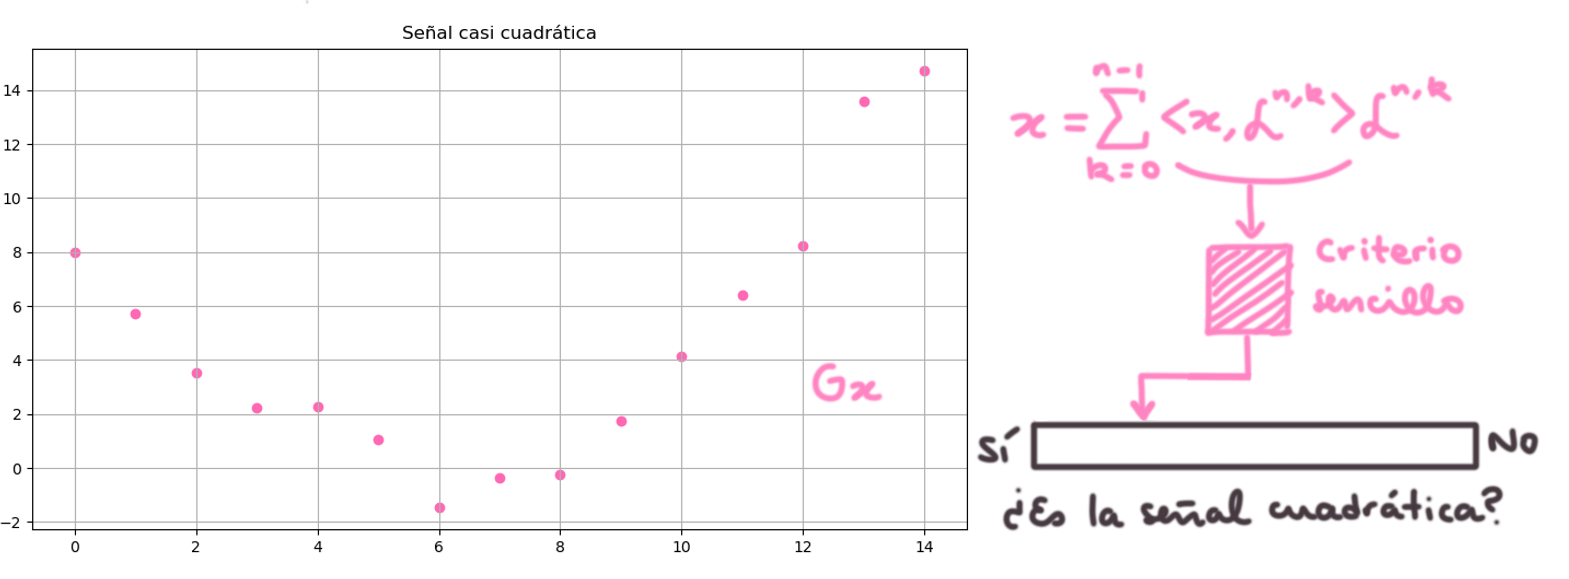
\includegraphics[width=0.95\linewidth]{cuadr2}
            \end{block}
            \vfill
            
  
			\begin{block}{Construcci\'on}
			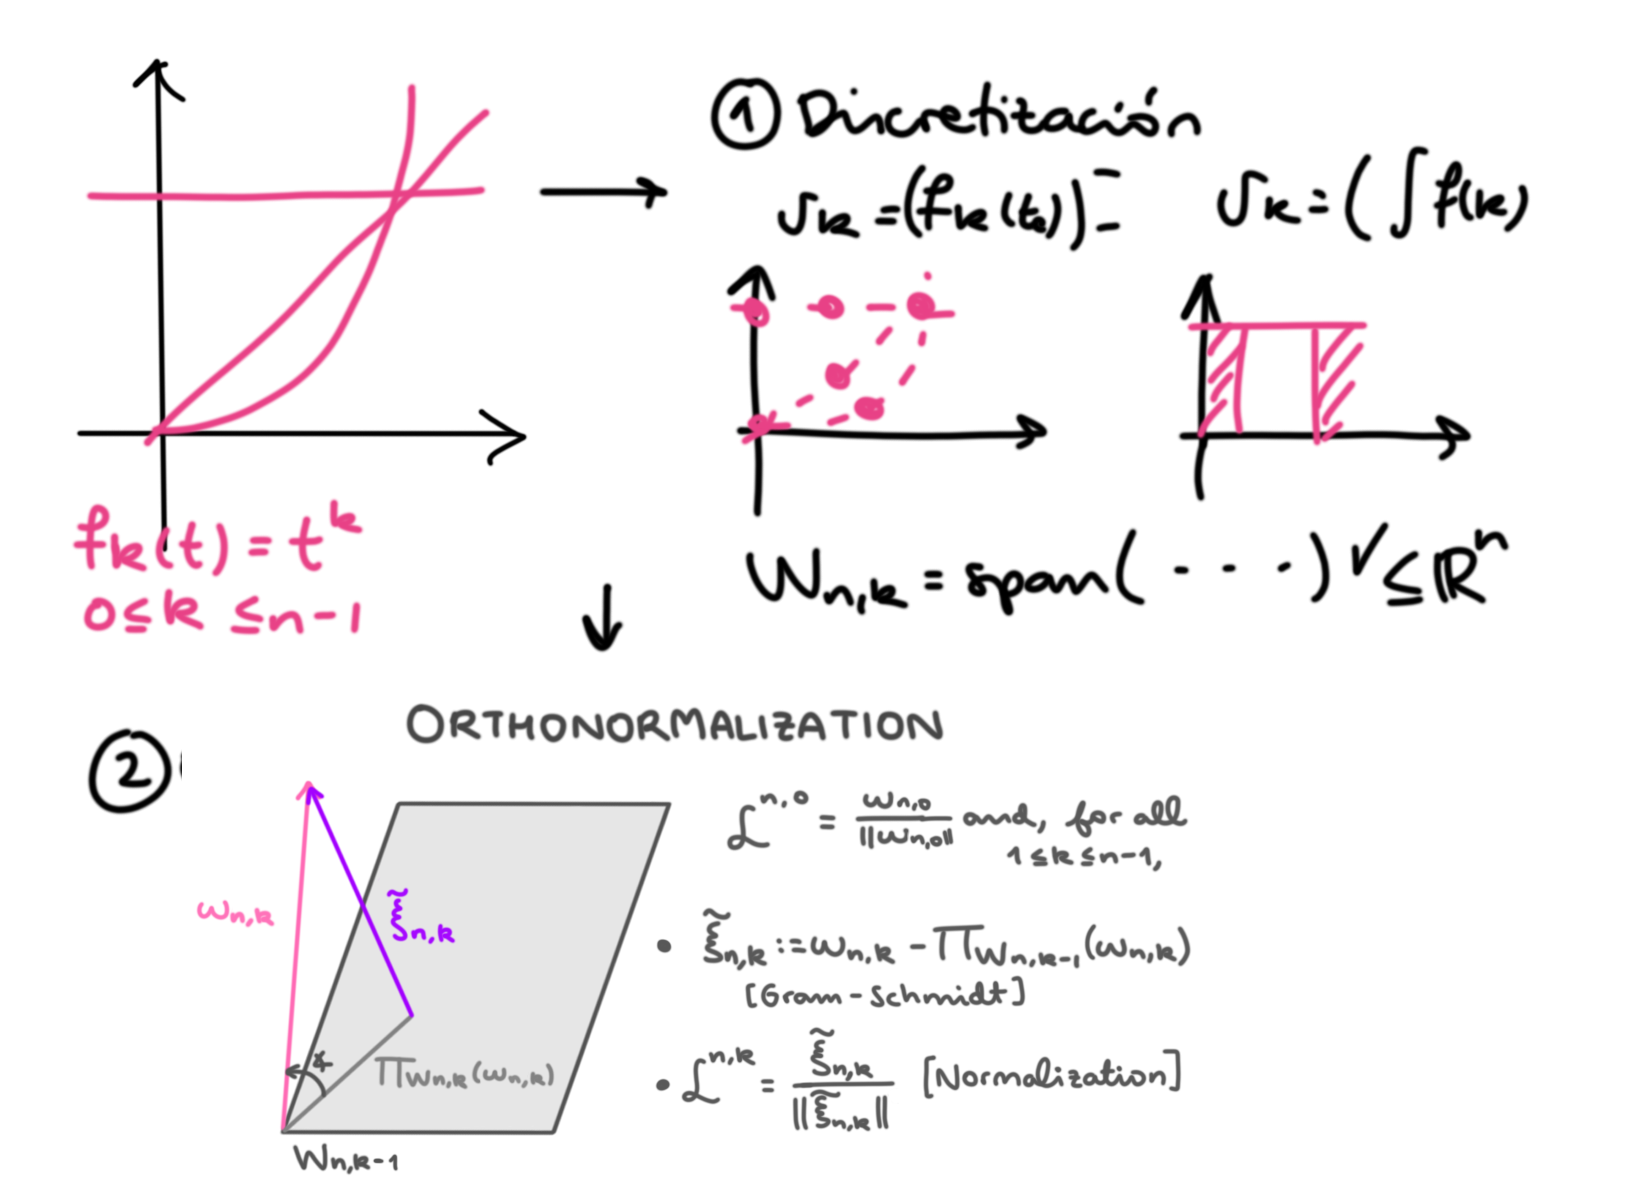
\includegraphics[width=0.95\linewidth]{esquema_construccion}	
			\end{block}			                        
            \vfill

            
            
			\begin{block}{Espacios de polinomios discretos }
			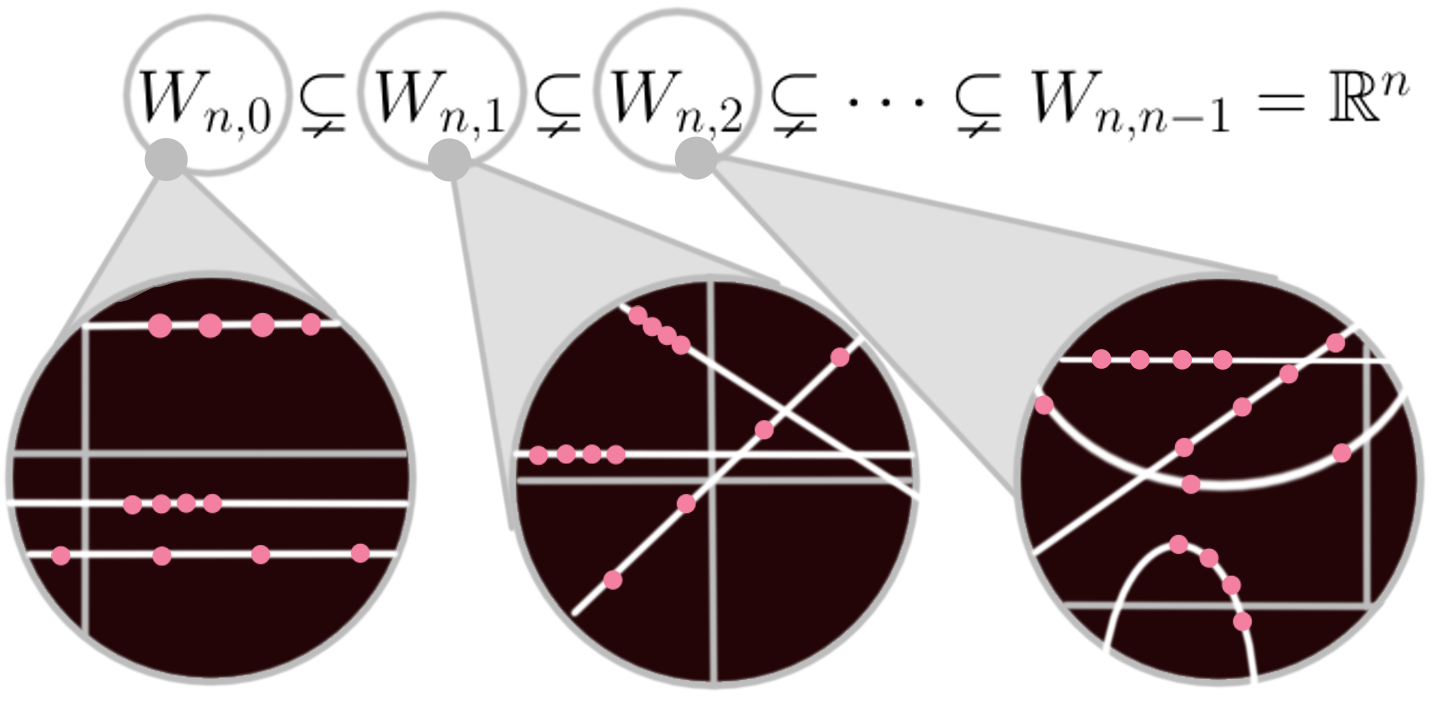
\includegraphics[width=0.7\linewidth]{nuevas_lupas}
			Noci\'on
			de grado para se\~nales $n-$dimensionales
			
			a\\
			a\\
			a\\
			a\\
			a\\
			a\\
			a\\
			a\\
			a\\
			a\\
			a\\
			a\\
			a\\
			\end{block}		
			\vfill	
			
			            

         % }
       % \end{minipage}
      \end{beamercolorbox}
    \end{column}
    % ---------------------------------------------------------%
    % end the column

    % ---------------------------------------------------------%
    % Set up a column 
    \begin{column}{.49\textwidth}
      %\begin{beamercolorbox}[center,wd=\textwidth]{postercolumn}
       % \begin{minipage}[T]{.95\textwidth} % tweaks the width, makes a new \textwidth
         % \parbox[t][\columnheight]{\textwidth}{ % must be some better way to set the the height, width and textwidth simultaneously
            % Since all columns are the same length, it is all nice and tidy.  You have to get the height empirically
            % ---------------------------------------------------------%

            \begin{block}{Results: Unaligned Faces}
              \begin{columns}
                \begin{column}{.59\textwidth}
                  \begin{itemize}
                  \item Automatically aligned by Viola \& Jones
                  \end{itemize}
                  \vskip-0.5ex
                  \begin{table}
                    \centering
                    \small
                    \begin{tabular}{@{} p{.4\linewidth} r r @{}}
                      \toprule 
                      Descriptor  &      \multicolumn{2}{c @{}}{Error Rates [\%]}      \\
                      \cmidrule(l){2-3}   
                      &   AR-Face       & CMU-PIE  \\
                      \cmidrule(r){1-1}  \cmidrule(lr){2-2}  \cmidrule(l){3-3}  
                      SURF-64     &   5.97          & 15.32    \\ 
                      SURF-128    &   5.71          & 11.42    \\ 
                      SIFT        &   5.45          & 8.32     \\  
                      \addlinespace
                      U-SURF-64   &   5.32          & 5.52     \\  
                      U-SURF-128  &   5.71          & \textbf{4.86}  \\ 
                      U-SIFT      &   \textbf{4.15} & 8.99     \\  
                      \bottomrule
                    \end{tabular}
                  \end{table}
                \end{column}
                \begin{column}{.39\textwidth}                
                  \vskip-3ex
                  \begin{itemize}
                  \item Manually aligned faces 

                      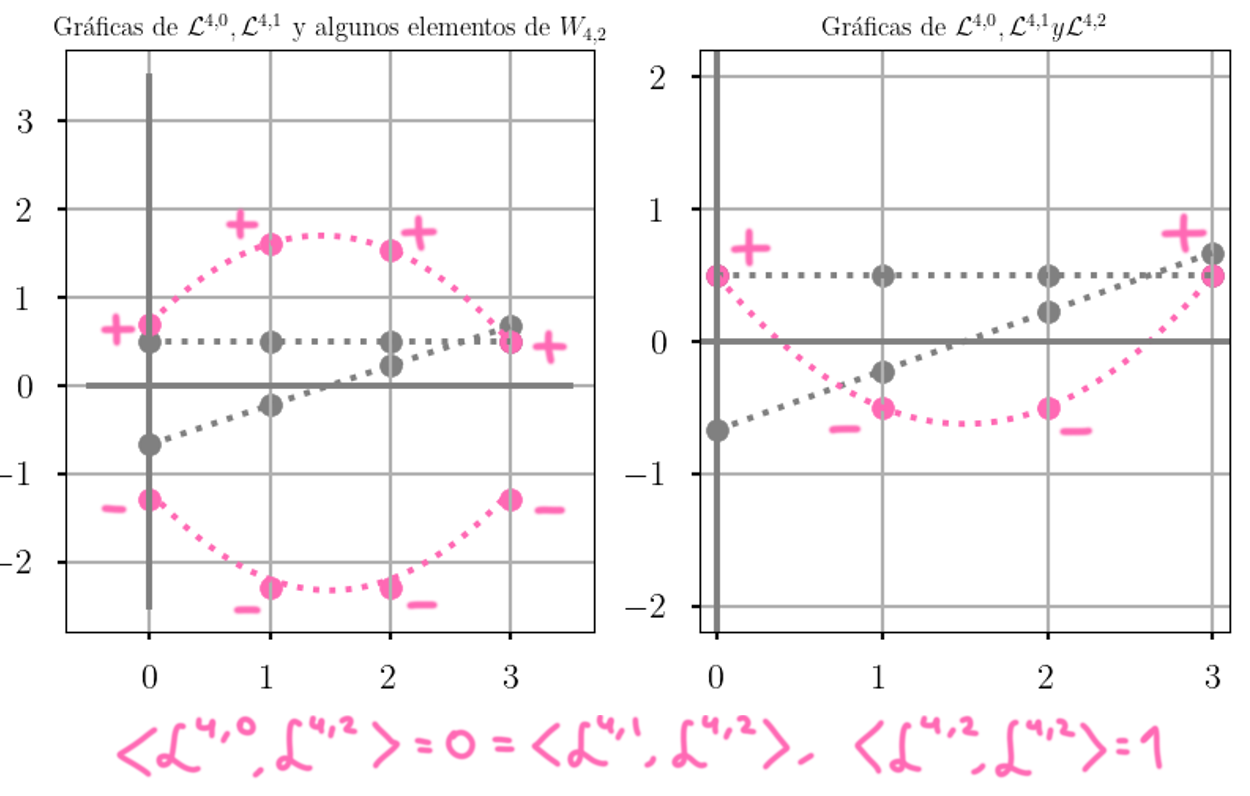
\includegraphics[width=0.9\linewidth]{oscil2}

                  \item Unaligned faces 

                      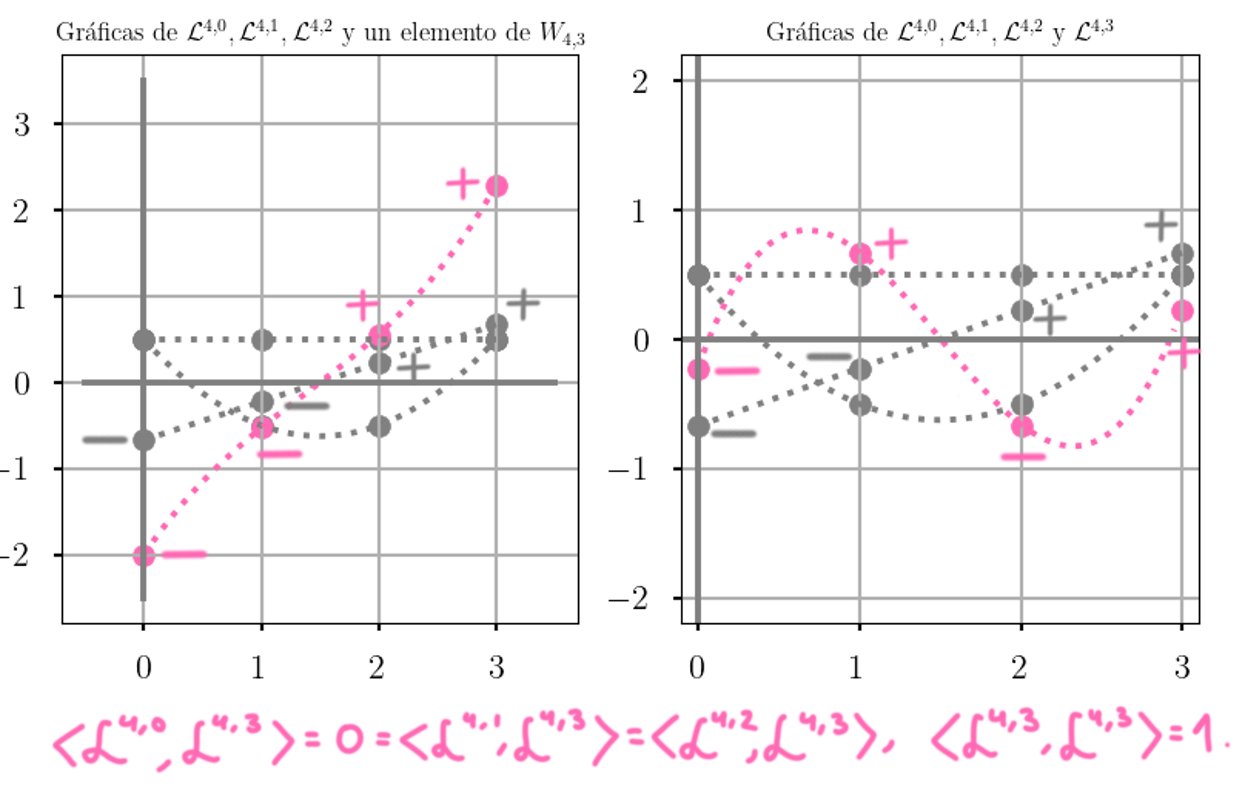
\includegraphics[width=0.9\linewidth]{oscil3}

                  \end{itemize}
                \end{column}
              \end{columns}
            \end{block}
            \vfill
            
            			\begin{block}{Construcci\'on}
			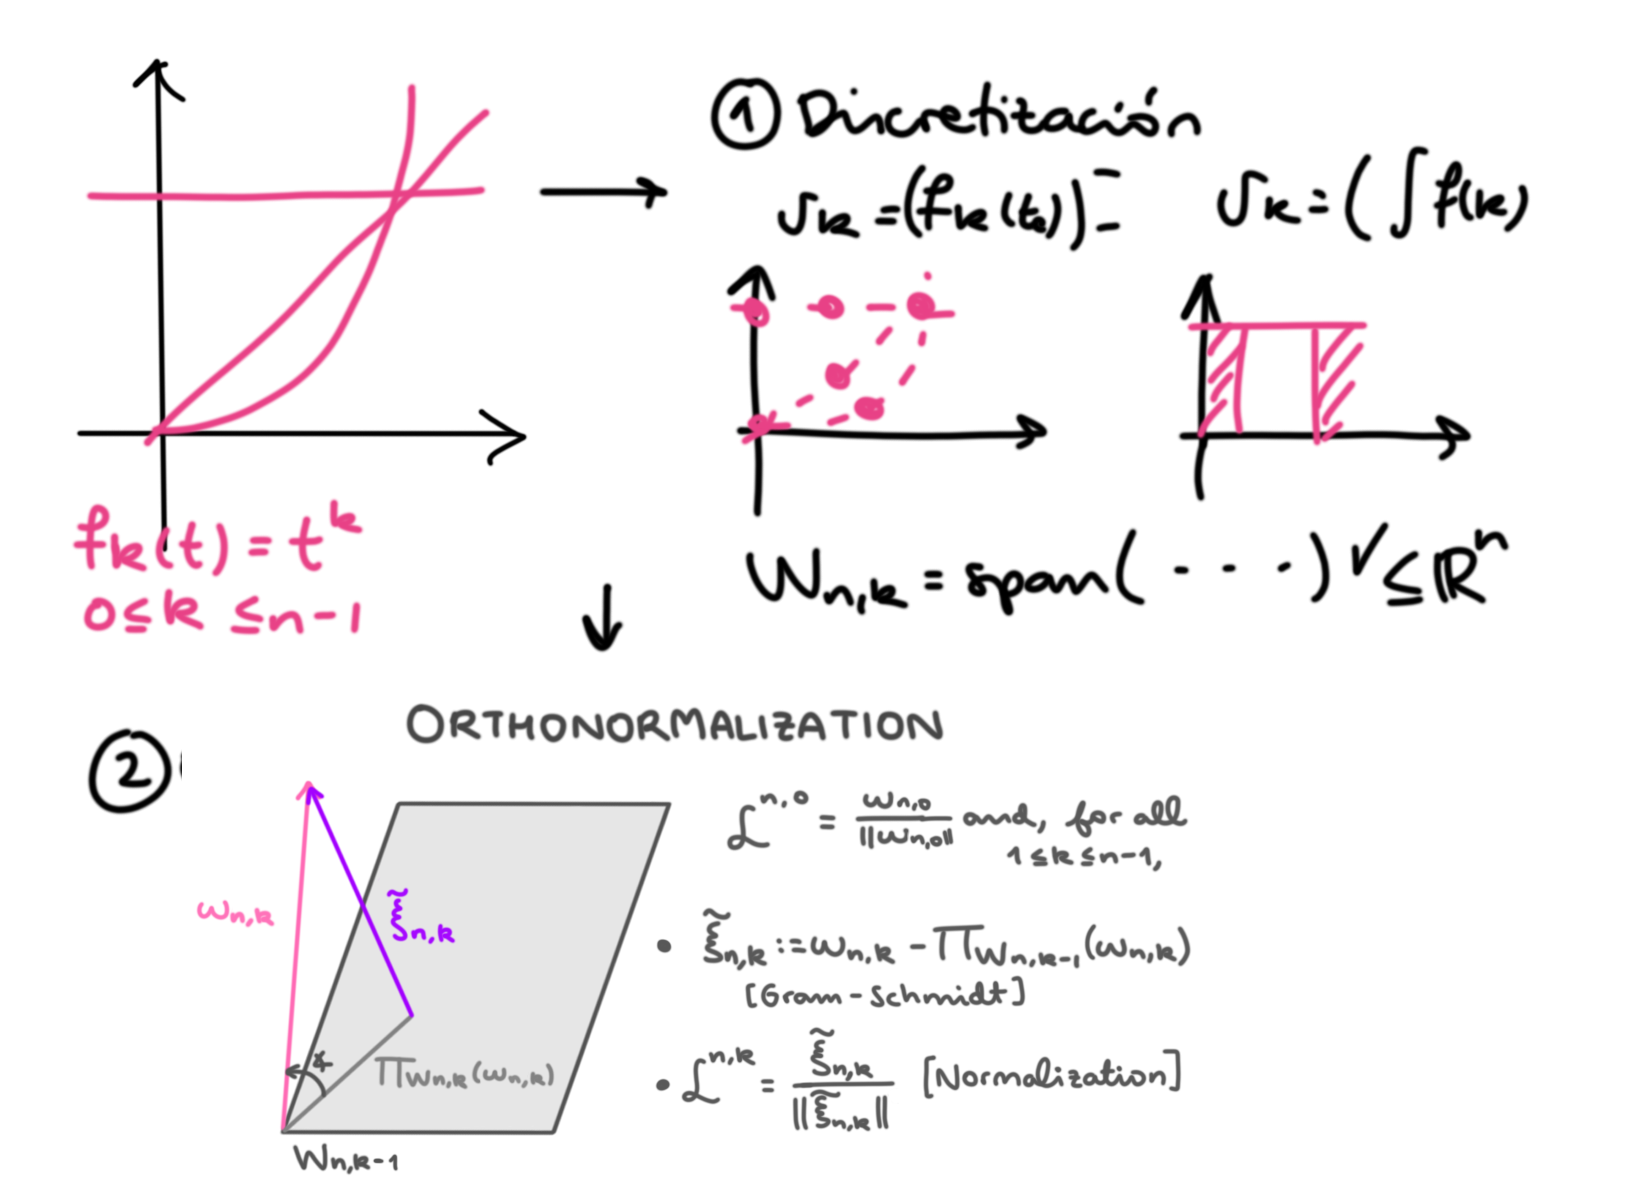
\includegraphics[width=0.95\linewidth]{esquema_construccion}	
			\end{block}			                        
            \vfill

            
            
			\begin{block}{Espacios de polinomios discretos }
			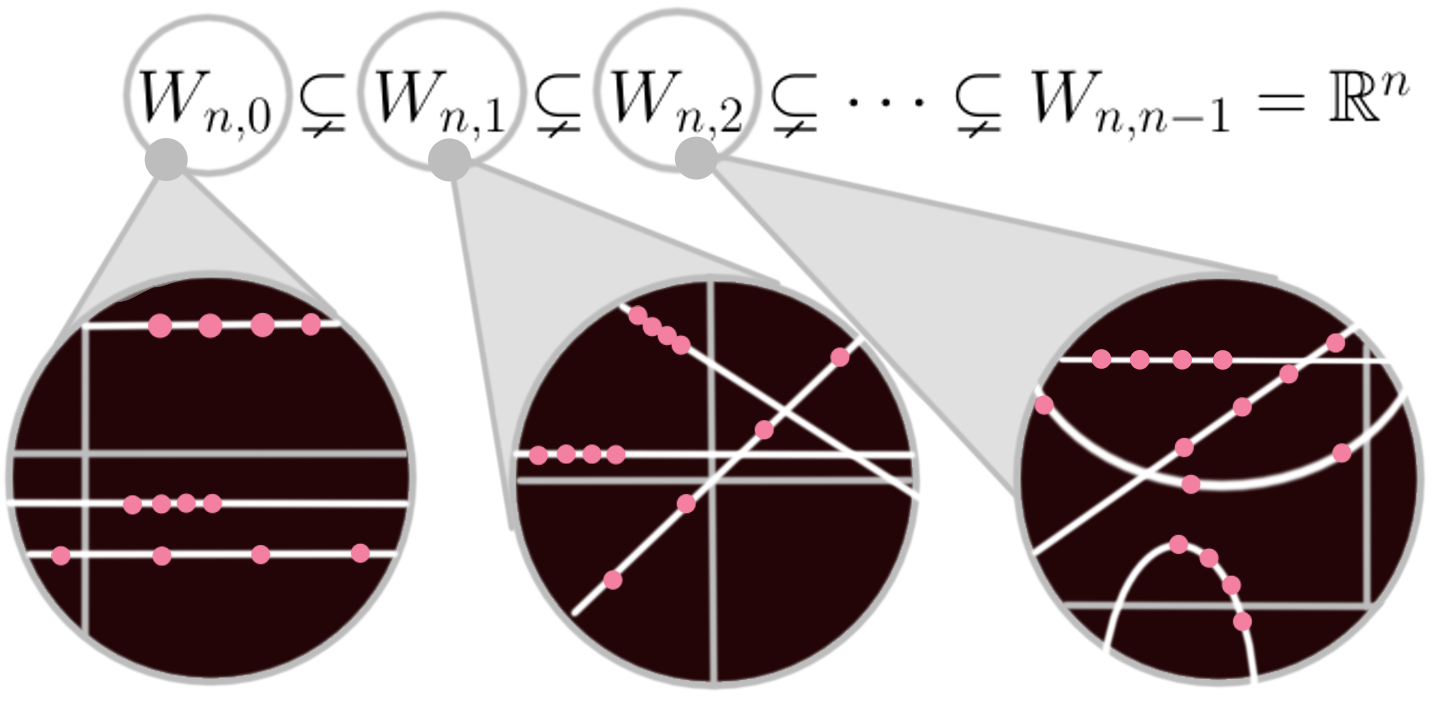
\includegraphics[width=0.7\linewidth]{nuevas_lupas}
			Noci\'on
			de grado para se\~nales $n-$dimensionales
			\end{block}		
			\vfill	
            
            
          %}
          % ---------------------------------------------------------%
          % end the column
        %\end{minipage}
      %\end{beamercolorbox}
    \end{column}
    % ---------------------------------------------------------%
    % end the column
  \end{columns}
  \vskip1ex
  %\tiny\hfill\textcolor{ta2gray}{Created with \LaTeX \texttt{beamerposter}  \url{http://www-i6.informatik.rwth-aachen.de/~dreuw/latexbeamerposter.php}}
  \tiny\hfill{Created with \LaTeX \texttt{beamerposter}  \url{http://www-i6.informatik.rwth-aachen.de/~dreuw/latexbeamerposter.php} \hskip1em}
\end{frame}
\end{document}

